\documentclass[main.tex]{subfiles}
\begin{document}
\chapter{Elementary trigonometry}
We have met the ideas of angles and distances. The subject of trigonometry allows us to convert between the two. For example, if we know that the wheel of a steam engine has turned one eight of a complete turn ($\pi/4$ radians) then how much forward or backward movement will the piston of the engine have moved?

``Trigonometry'' literally means (from Greek) the measurement of triangles (``trigons'' though we don't call them that). In a way the name undersells its usefulness. In a sense you can use trigonometry even if there are no triangles around, although of course if there are at least three points in any problem you can always draw a triangle in to connect them.

Let us start with a simple example of the problem that we want to solve. Let us imagine that the circle depicted in figure \ref{fig:sine1} is vertical. $O$ is the centre of the circle. The line passing horizontally through the circle we can take, arbitrarily, as our zero height line. If it helps to think of it as ``ground level'' then that is fine. The line $OP$ is something that is rotating in that vertical plane. It might be an abstraction of (say) the arm of a crane, or a rocket launching vehicle.

Let us suppose that the arm has rotated through an angle $\theta$. How high will the end of the arm (point $P$) be above the baseline. 

\begin{figure}[H]
  \label{fig:sine1}
  \begin{tikzpicture}
    \coordinate (O) at (0,0);
    \coordinate (P) at (3.2, 2.4); %(1.6, 1.2);
    \coordinate (hhtop) at (6, 2.4);

    \fill (O) circle [radius=3pt];
    \fill (P) circle [radius=3pt];
    
    \draw (-6,0) -- (O) node [below left]{O} -- (6,0);
    \draw [<->] (6,0) -- node [right] {how high?}(hhtop);
    \draw (O) -- (P) node [above right]{P};
    \draw [dotted] (P) -- (hhtop);
    \draw (O) circle (4);
  \end{tikzpicture}
  \caption{How high is P?}
  
\end{figure}

Well without more information this question is unanswerable because it depends on the size of the circle as well as the angle of $OP$ from the ``horizontal''. 

As it happens the size of the circle is not really critical, because if we scale up the size of the circle, we scale the height of $P$ by the same amount. We might just as well work out the example for a circle with radius of $1$. Once we have the answer, we can just multiply it by the radius if the circle we are interested in.

If you aren't happy with the idea that everything just scales up, I will prove it in the end notes of this chapter using similar triangles.

Even though we don't (yet) know exactly how the height of $P$ behaves as it moves around the circle, there are a few things we do know. Let us draw a picture with four points ($A, B, C, D$) marked around it at the obvious four cardinal points of the circle and consider what happens to P's height as it travels around the circle. Mathematicians traditionally measure angles anticlockwise\footnote{why?}.

\begin{figure}[H]
  \label{fig:sine1}
  \begin{tikzpicture}
    \coordinate (O) at (0,0);
    \coordinate (P) at (3.2, 2.4); %(1.6, 1.2);
    \coordinate (hhtop) at (6, 2.4);
    \coordinate (A) at (4, 0);
    \coordinate (B) at (0, 4);
    \node at (0, 4.3) {B};
    \node [below] (D) at (0, -4) {D};
    \coordinate (C) at (-4, 0);
    \coordinate (D) at (0, -4);

    \fill (O) circle [radius=3pt];
    \fill (P) circle [radius=3pt];
    \fill (A) circle [radius=3pt];
    \fill (B) circle [radius=3pt];
    \fill (C) circle [radius=3pt];
    \fill (D) circle [radius=3pt];
    
    \draw (-6,0) -- (C) node [above left] {C} -- (O) node [below left]{O} -- (A) node [above right] {A} -- (6,0);
    \draw [<->] (6,0) -- node [right] {how high?}(hhtop);
    \draw (O) -- (P) node [above right]{P};
    \draw [dotted] (P) -- (hhtop);
    \draw (O) circle (4);

    \pic [draw, ->, "$\theta$", ultra thick, angle eccentricity=1.5, angle radius=1.5cm] {angle = A--O--P};

  \end{tikzpicture}
  \caption{P's journey around the circle}
  
\end{figure}

When $P$ starts out at $A$, it clearly has a height of zero. As it rotates anticlockwise, the height will increase until it reaches a maximum at $B$. At this point $\theta=\pi/2 \text{radians}$. Since the circle has radius $1$ (known in the trade as a ``unit circle''), that maximum is $1$. 

Further round the circle, between $\pi/2$ and $\pi$ radians, the height declines until at $C$ (where $\theta=\pi$) the height is zero.

Further around the circle the arm is going to go below ground level. We can imagine that it is able to do so because someone has dug a ditch (not illustrated). Maybe it is the digging arm of a digger doing just that. The sensible thing to do here is treat the height of $P$ as negative, because it is below our chosen zero. 

Thus $P$ then becomes negative from $\theta=\pi$ until $\theta=3\pi/2$ at which point it has reached its minimum height $-1$. After this $P$ begins to move back up until it arrives back at $A$. It should be clear that if $\theta$ grows beyond $2\pi$ the whole process will simply be repeated.

If we draw a graph of the height of $P$ against the angle, this pattern becomes clearer.

\begin{figure}[H]
  \label{fig:sinegraph1}
    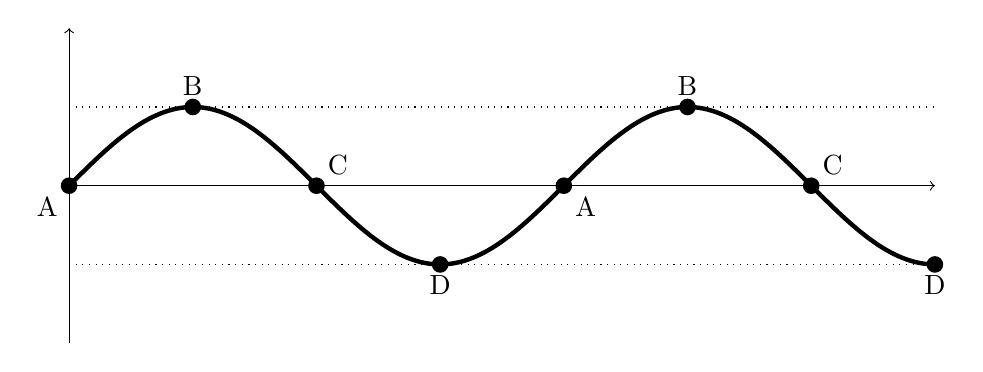
\begin{tikzpicture}

    \draw [->] (0,0) -- (10.9956, 0);
    \draw [->] (0, -2) -- (0, 2);
    \draw [dotted] (0, 1) -- (10.9956, 1);
    \draw [dotted] (0, -1) -- (10.9956, -1);
    \fill (0,0) circle [radius=3pt];
    \fill (1.571,   1) circle [radius=3pt];
    \fill (3.1416,  0) circle [radius=3pt];
    \fill (4.7124, -1) circle [radius=3pt];
    \fill (6.2832,  0) circle [radius=3pt];
    \fill (7.8540,  1) circle [radius=3pt];
    \fill (9.4248,  0) circle [radius=3pt];
    \fill (10.9956,-1) circle [radius=3pt];
    \draw [ultra thick] (0,0) node [below left]{A} sin (1.571, 1) node [above] {B} cos (3.1416, 0) node [above right] {C} sin (4.7124, -1) node [below] {D} cos (6.2832, 0) node [below right] {A} sin (7.8540, 1) node [above] {B} cos (9.4248, 0) node [above right] {C} sin (10.9956, -1) node [below] {D};
  \end{tikzpicture}
  \caption{The true sine - a folding line}
  
\end{figure}

Figure (\ref{fig:sinegraph1}) shows a graph of height against angle. The rather beautiful shape of the line inspired an Arabic name for the function {\emph jaib} meaning a fold. Translated into Latin by mediaeval writers this became {\emph sinus}. In modern mathematical writing this has become ``sine'' and the sine of the angle $\theta$ is usually written $sin \theta$.

Many graphs of sine (in textbooks too I am afraid) deliberately stretch the y-axis so as to butch up the curve to make it look like a steeper wave, but figure (\ref{fig:sinegraph1}) is as near to scale as I can make it and illustrates just how smoothly the curve rises and falls. It is one of the most beautiful shapes in mathematics or physics.

Armed with this new name, we can answer the question in figure \ref{fig:sine1}.

\begin{figure}[H]
  \label{fig:sinename}
  \begin{tikzpicture}
    \coordinate (O) at (0,0);
    \coordinate (P) at (3.2, 2.4); %(1.6, 1.2);
    \coordinate (hhtop) at (6, 2.4);
    \coordinate (A) at (4, 0);
    \coordinate (B) at (0, 4);
    \node at (0, 4.3) {B};
    \node [below] (D) at (0, -4) {D};
    \coordinate (C) at (-4, 0);
    \coordinate (D) at (0, -4);

    \fill (O) circle [radius=3pt];
    \fill (P) circle [radius=3pt];
    \fill (A) circle [radius=3pt];
    \fill (B) circle [radius=3pt];
    \fill (C) circle [radius=3pt];
    \fill (D) circle [radius=3pt];
    
    \draw (-6,0) -- (C) node [above left] {C} -- (O) node [below left]{O} -- (A) node [above right] {A} -- (6,0);
    \draw [<->] (6,0) -- node [right] {$\sin\theta$}(hhtop);
    \draw (O) -- (P) node [above right]{P};
    \draw [dotted] (P) -- (hhtop);
    \draw (O) circle (4);

    \pic [draw, ->, "$\theta$", ultra thick, angle eccentricity=1.5, angle radius=1.5cm] {angle = A--O--P};

  \end{tikzpicture}
  \caption{The definition of sine}
\end{figure}

Another equally interesting distance to work out would be how far $P$ has stretched out horizontally. So useful was this value that it was given a name the ``cosine'' because it is a companion of the sine. 

% picture of cosine
Cosine is in fact our friend since in disguise. If you turn figure ???? on its side you can see that cosine is, in some sense, the same function as sine only $\pi/2$ ahead of it. This becomes clear if we plot cosine and sine on the same graph;

% sine and cosine graph.

It should be clear from the graph (and the definition) that 
$$\sin(\theta) = \cos(\theta + \pi/2)$$

%the effect of the radius.

%Cartesian co-ordinates. Transforming between polar and cartesian.
% using it to work out distance of stars, parallax
% surveying

% use it for cords of circles?

\subsection{The Tangent}
%intro. Shadows motivation.
%two ways to define tan
% picture with tan and secant
% different behaviour, infinite, graph
% the secant
%identities

$$\sec^2 + 1= \tan^2$$

%the cotangent and cosecant.
% more identities

%triangles, socatoa and so on
% CAST and sign of them


\subsection{Obscure trigonometrical functions}

% rest of functions.

\end{document}

%%  LocalWords:  trigons
